% Benchmark Evaluation Section

In order to demonstrate the capabilities of the CircusTent benchmark suite, in this section we conduct an evaluation of atomic memory operations on a variety of different test platforms.
We first introduce our test platforms and briefly describe pertinent details of their underlying architecture in section ~\ref{subsec:platforms}.
We next detail our evaluation methodology in section ~\ref{subsec:methodology}.
Finally, we present and discuss the our evaluation results for each of the CircusTent kernels in section ~\ref{subsec:results}.

\subsection{Platforms}
\label{subsec:platforms}

We evaluate CircusTent across a total of fourteen different platforms.
The platforms encompass a variety of different device classes/architectures that include embedded, laptop, desktop, server, and petascale class supercomputers.
Further, the processors utilized encompass a variety of different instruction set architectures from Intel, AMD, and ARM.
These systems feature both single and dual socket systems whose processors have varied core counts and clock speeds.
Further, the complexity of these system's memory subsystem and cache hierarchy are similar varied.

However, using CircusTent and our normalized GAMs metric, we are able to directly compare the performance of these memory hierarchies with respect to atomic operations in a variety of different scenarios. (using memory access patterns common in...).
Table ~\ref{tab:benchsys} provides an overview of our test platforms specifications wherein each system is denoted by its processor.
In addition, we also provide a brief description of each platform in the list below.
In particular, we detail the implementation of each platform's cache hierarchy as this directly correlates to its shared memory performance. 

\begin{table*}
\caption{Benchmark System Configurations}
\label{tab:benchsys}
\begin{tabular}{ccccp{15mm}ccp{16mm}c}
\toprule
System&Clock Frequency&Cores / Socket&Total Sockets&LLC Size\newline~/ Socket&Total Memory&Array Size&Operating\newline System&Compiler\\
\midrule
Cortex-A53      & 1.40Ghz & 4  & 1 & 64KiB  & 512MiB & 256MiB  & Ubuntu\newline 18.04 4.15.0 & GCC 7.4.0\\
Cortex-A72      & 1.50Ghz & 4  & 1 & 1MiB   & 4GiB & 256MiB  & Debian\newline 10.1 4.19.75 & GCC 8.3.0\\
Ryzen V1605B    & 1.58Ghz & 4  & 1 & 4MiB    & 32GiB & 15GiB & Ubuntu\newline 19.04 5.2.10&GCC 8.3.0\\
Opteron 4130    & 2.60Ghz & 4  & 2 & 6MiB   & 64GiB & 15GiB & Centos7\newline 3.10.0&GCC 8.3.1\\
Core i5-3210M   & 2.50Ghz & 2  & 1 & 3MiB   & 4GiB & 256MiB & macOS\newline 10.13.6&clang 9.1.0\\
Core i7-3930K   & 3.20Ghz & 6  & 1 & 12MiB  & 64GiB & 15GiB & Linux Mint\newline 18.3 4.15.0&GCC 5.4.0\\
Core i7-4980HQ  & 2.80Ghz & 4  & 1 & 6MiB L3 +\newline 128MiB L4 & 16GiB & 15GiB & macOS\newline 10.15.3&GCC 9.2.0\\
Xeon Phi 7250   & 1.40Ghz & 68 & 1 & 16GiB \newline MCDRAM & 96GiB & 15GiB & SLES\newline 4.12.14&GCC 8.3.0\\
Xeon E5620      & 2.40Ghz & 4  & 2 & 12MiB & 48GiB & 15GiB & Ubuntu\newline 16.04 4.4.0&GCC 5.4.0\\
Xeon X5650      & 2.67Ghz & 6  & 2 & 12MiB & 64GiB & 15GiB & Ubuntu\newline 18.04 4.15.0&GCC 7.5.0\\
Xeon E5-2620 v3 & 2.40Ghz & 6  & 1 & 15MiB & 64GiB & 15GiB & Ubuntu\newline 16.04 4.4.0&GCC 5.4.0\\
Xeon E5-2670 v2 & 2.50Ghz & 10 & 2 & 25MiB & 64GiB & 15GiB & Centos7\newline 3.10.0&GCC 7.3.0\\
Xeon E5-2695 v4 & 2.10Ghz & 18 & 2 & 45MiB & 192GiB & 15GiB & Centos7\newline 3.10.0&GCC 7.3.0\\
Xeon E5-2698 v3 & 2.30Ghz & 16 & 2 & 40MiB & 128GiB & 15GiB & SLES\newline 4.12.14&GCC 8.3.0\\
\bottomrule
\end{tabular}
\end{table*}

\todo[inline]{Double check system specs and array sizes with John}

\subsection{Methodology}
\label{subsec:methodology}

Consistent with previous studies, we focus on evaluating the CircusTent suite in a shared-memory environment in this work\cite{}.
In order to do so, we execute each of the CircusTent kernels, detailed in section ~\ref{subsec:algorithms}, on the test platforms introduced above using the OpenMP-based CircusTent benchmark implementation. For each kernel, we conduct trials using both the atomic \textit{Add} and \textit{Compare-and-Swap} implementations.
For both versions, 64-bit operands are used throughout the evaluation to prevent any inconsistencies.
For the StrideN kernel, a uniform unit stride size of 9 is utilized for each trial.

We collect performance results on each platform.
In order to eliminate any performance variability associated with simultaneous multithreading (SMT), we vary the thread count from a single thread up to one thread per physical core for each platform.
Moreover, to better simulate real-world behavior, we allow the operating system and programming model to perform the mapping of threads to processor cores.

Where feasible, a uniform size of approximately 15 GiB is utilized for the \texttt{VAL} array on each platform. For the Cortex A-53, Cortex A-72, and Core i5-3210M systems, wherein physical memory limitations make this configuration impractical, a size of 256 MiB is utilized instead.
In order to generate sufficient runtime such that the benchmark's behavior normalizes, twenty million iterations are run as part of each trial conducted for each kernel.

\todo[inline]{Add previous shared-memory references}

\subsection{Results}
\label{subsec:results}

\begin{figure}[!t]
\centering
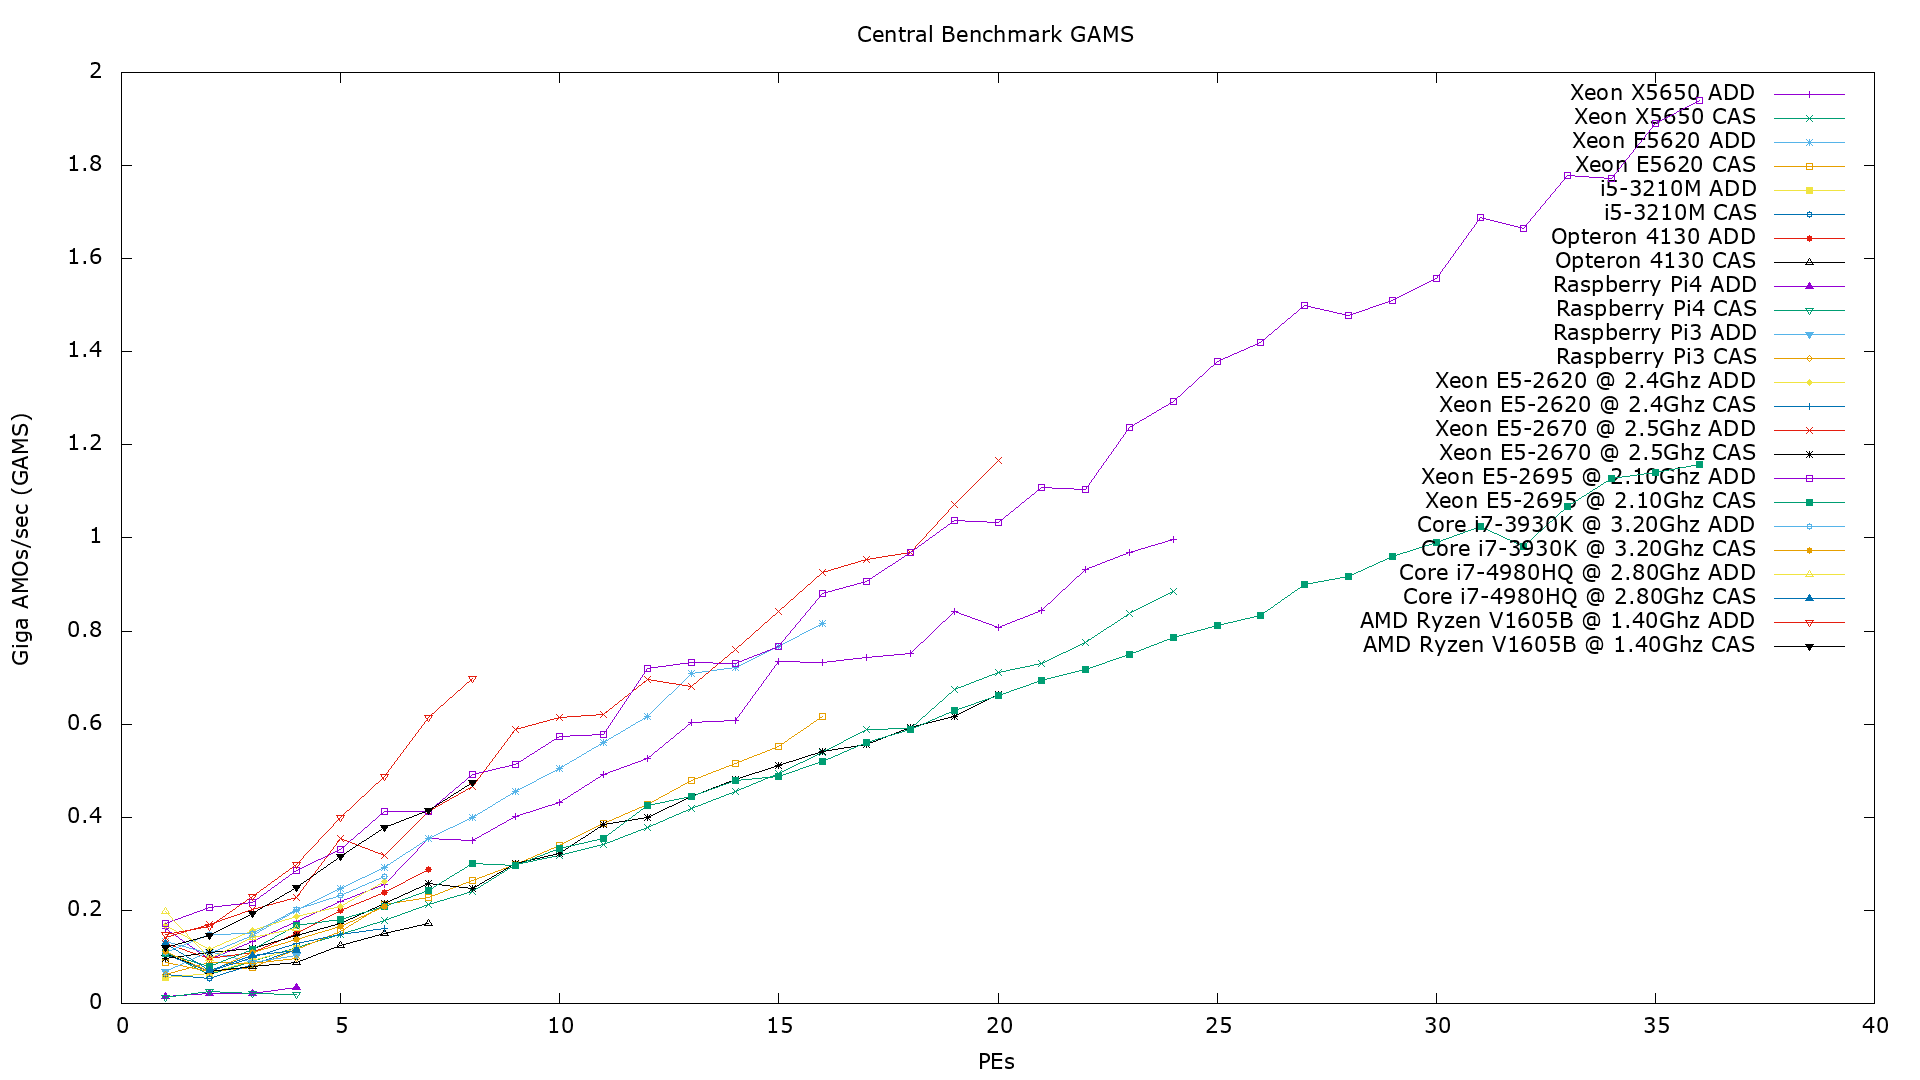
\includegraphics[width=3.5in]{figures/CENTRAL_GAMS.png}
\caption{Central Benchmark GAMS}
\label{fig:central_gams}
\end{figure}

\begin{figure}[!t]
\centering
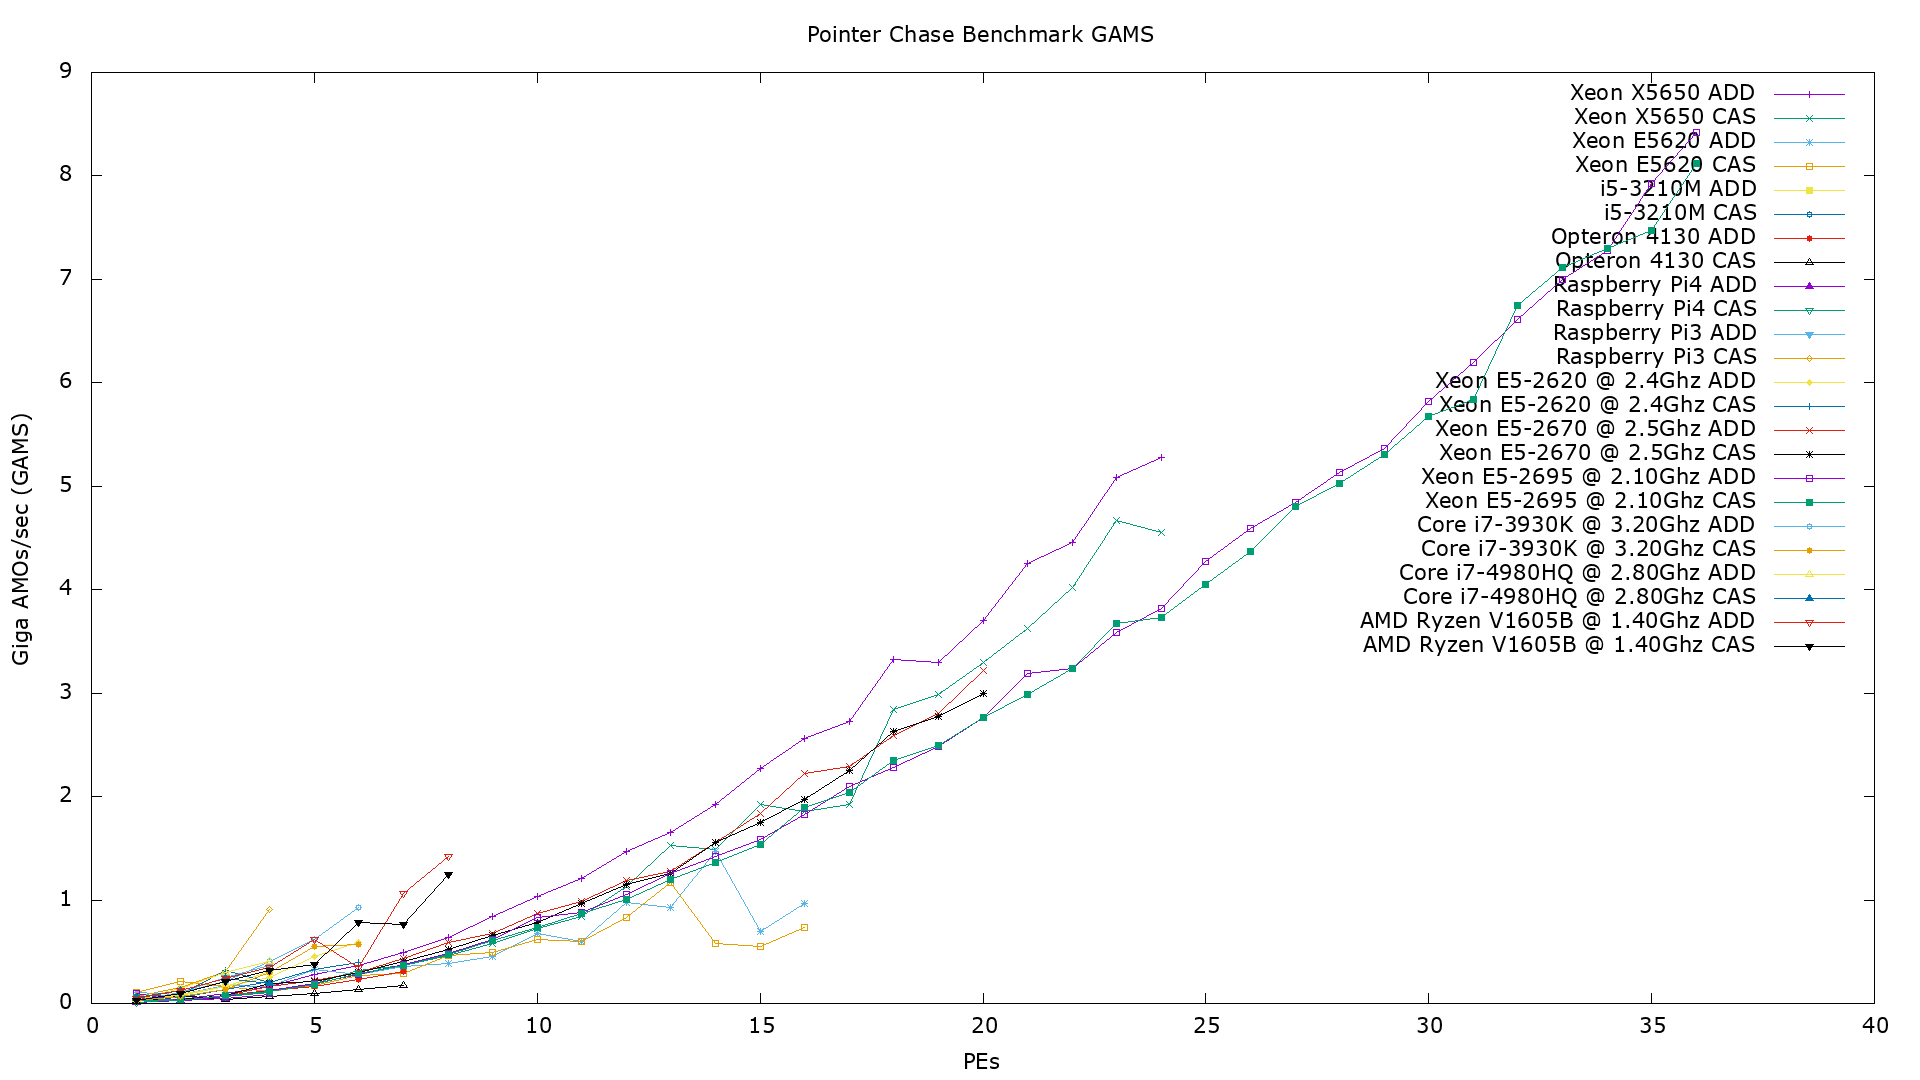
\includegraphics[width=3.5in]{figures/PTRCHASE_GAMS.png}
\caption{Pointer Chase Benchmark GAMS}
\label{fig:ptrchase_gams}
\end{figure}

\begin{figure}[!t]
\centering
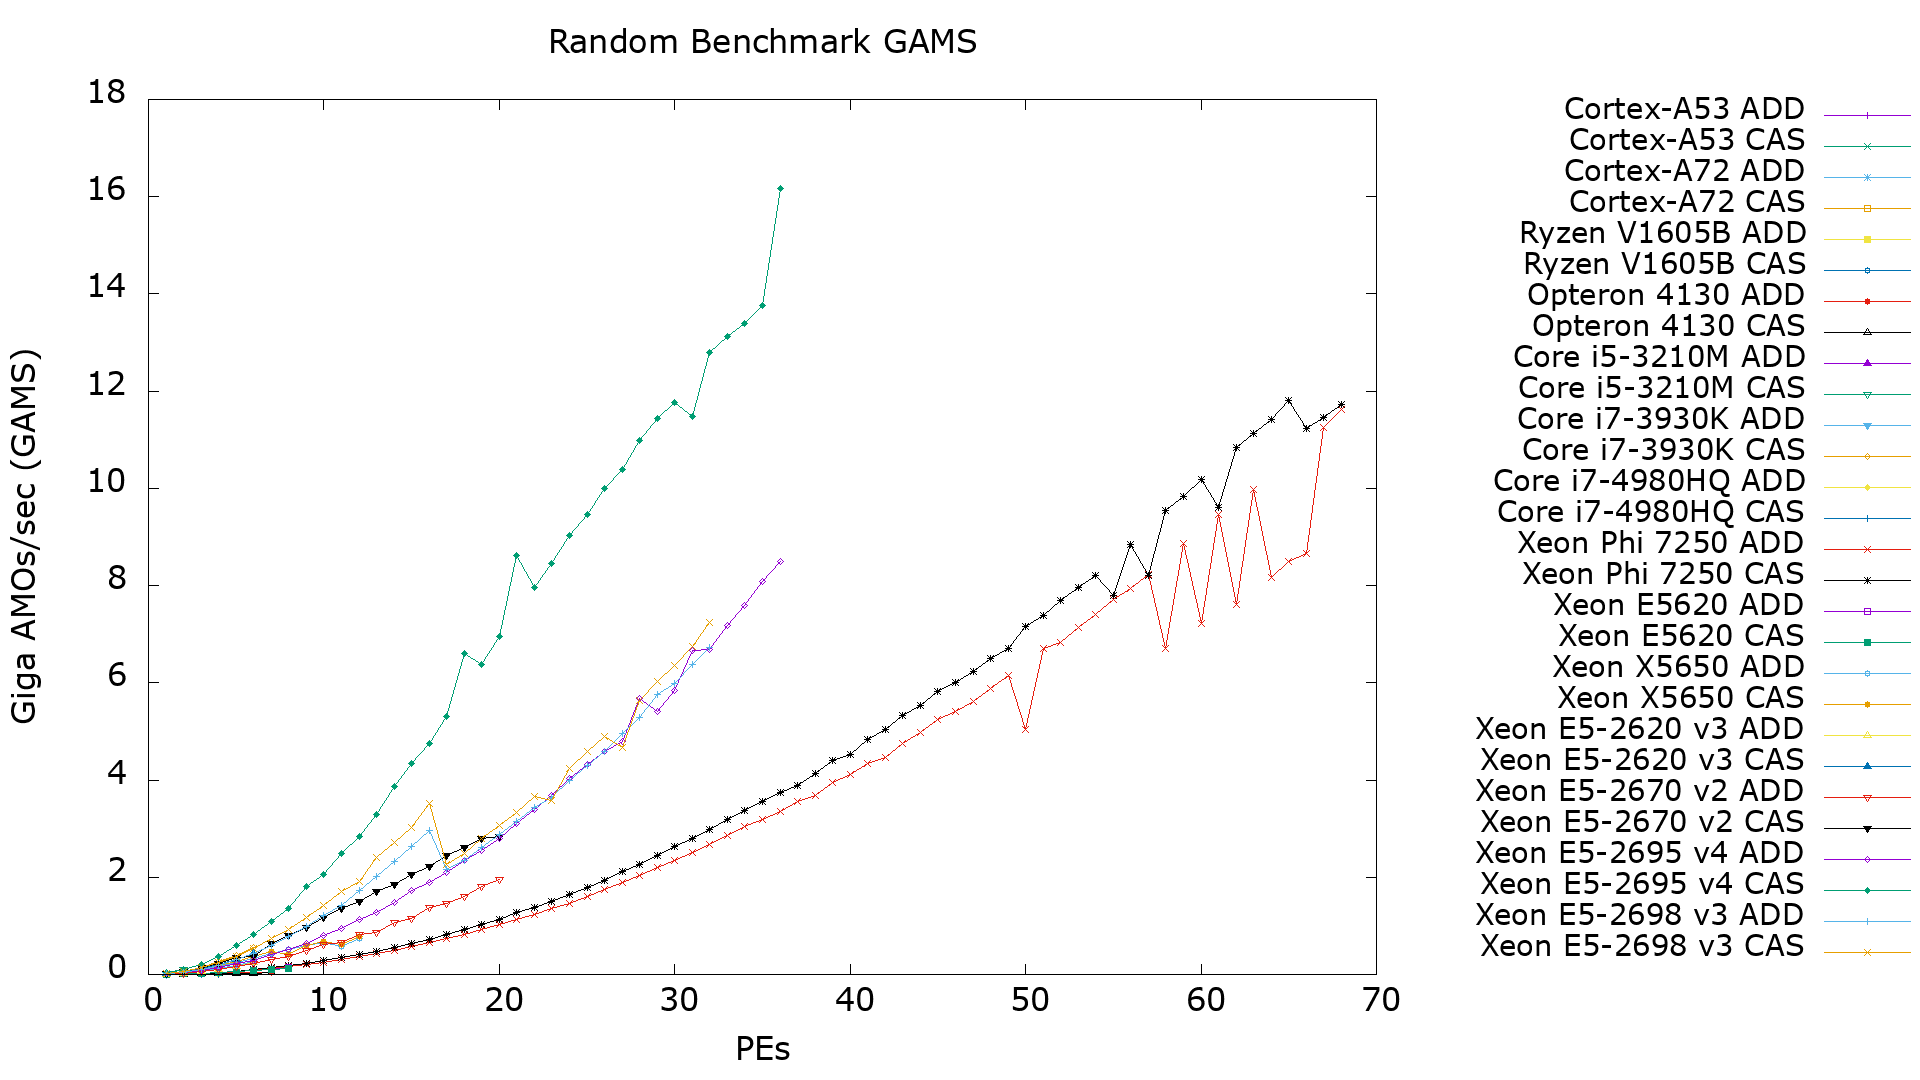
\includegraphics[width=3.5in]{figures/RAND_GAMS.png}
\caption{Random Benchmark GAMS}
\label{fig:rand_gams}
\end{figure}

\begin{figure}[!t]
\centering
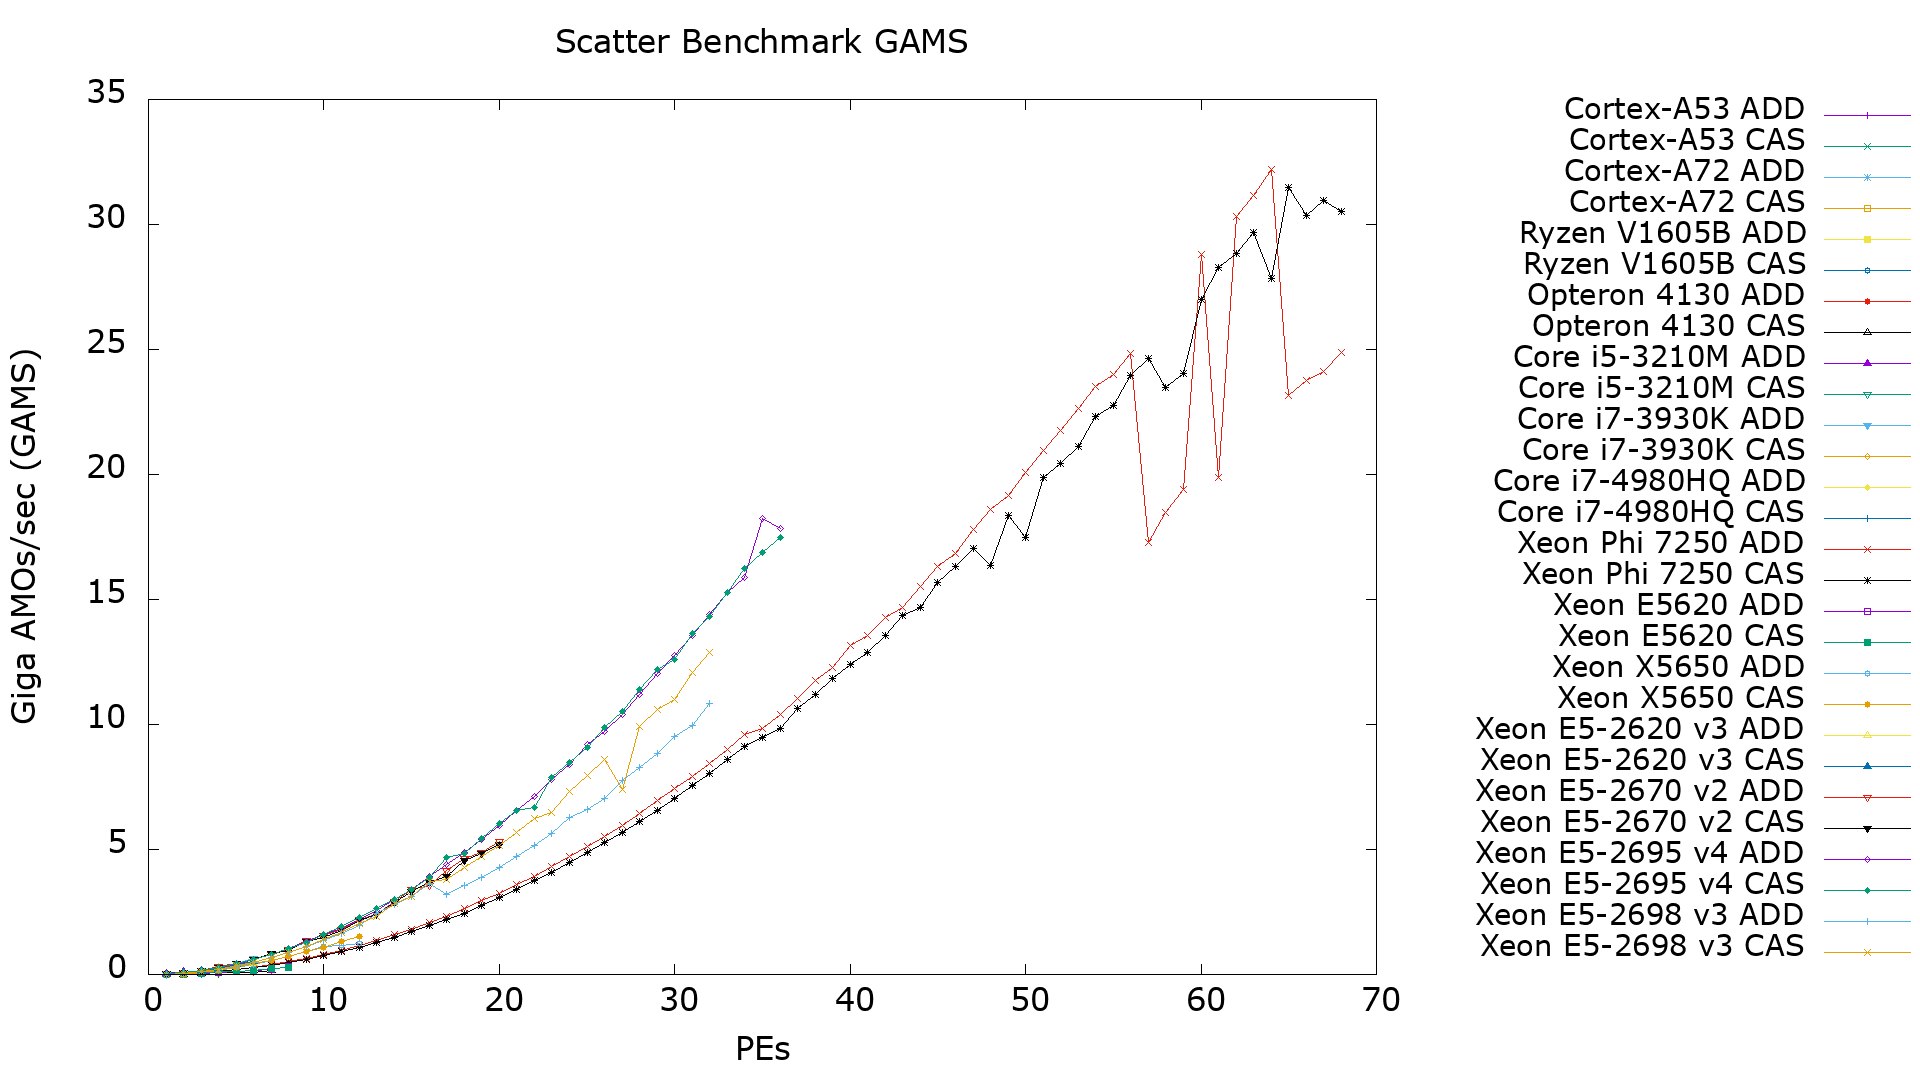
\includegraphics[width=3.5in]{figures/SCATTER_GAMS.png}
\caption{Scatter Benchmark GAMS}
\label{fig:scatter_gams}
\end{figure}

\begin{figure}[!t]
\centering
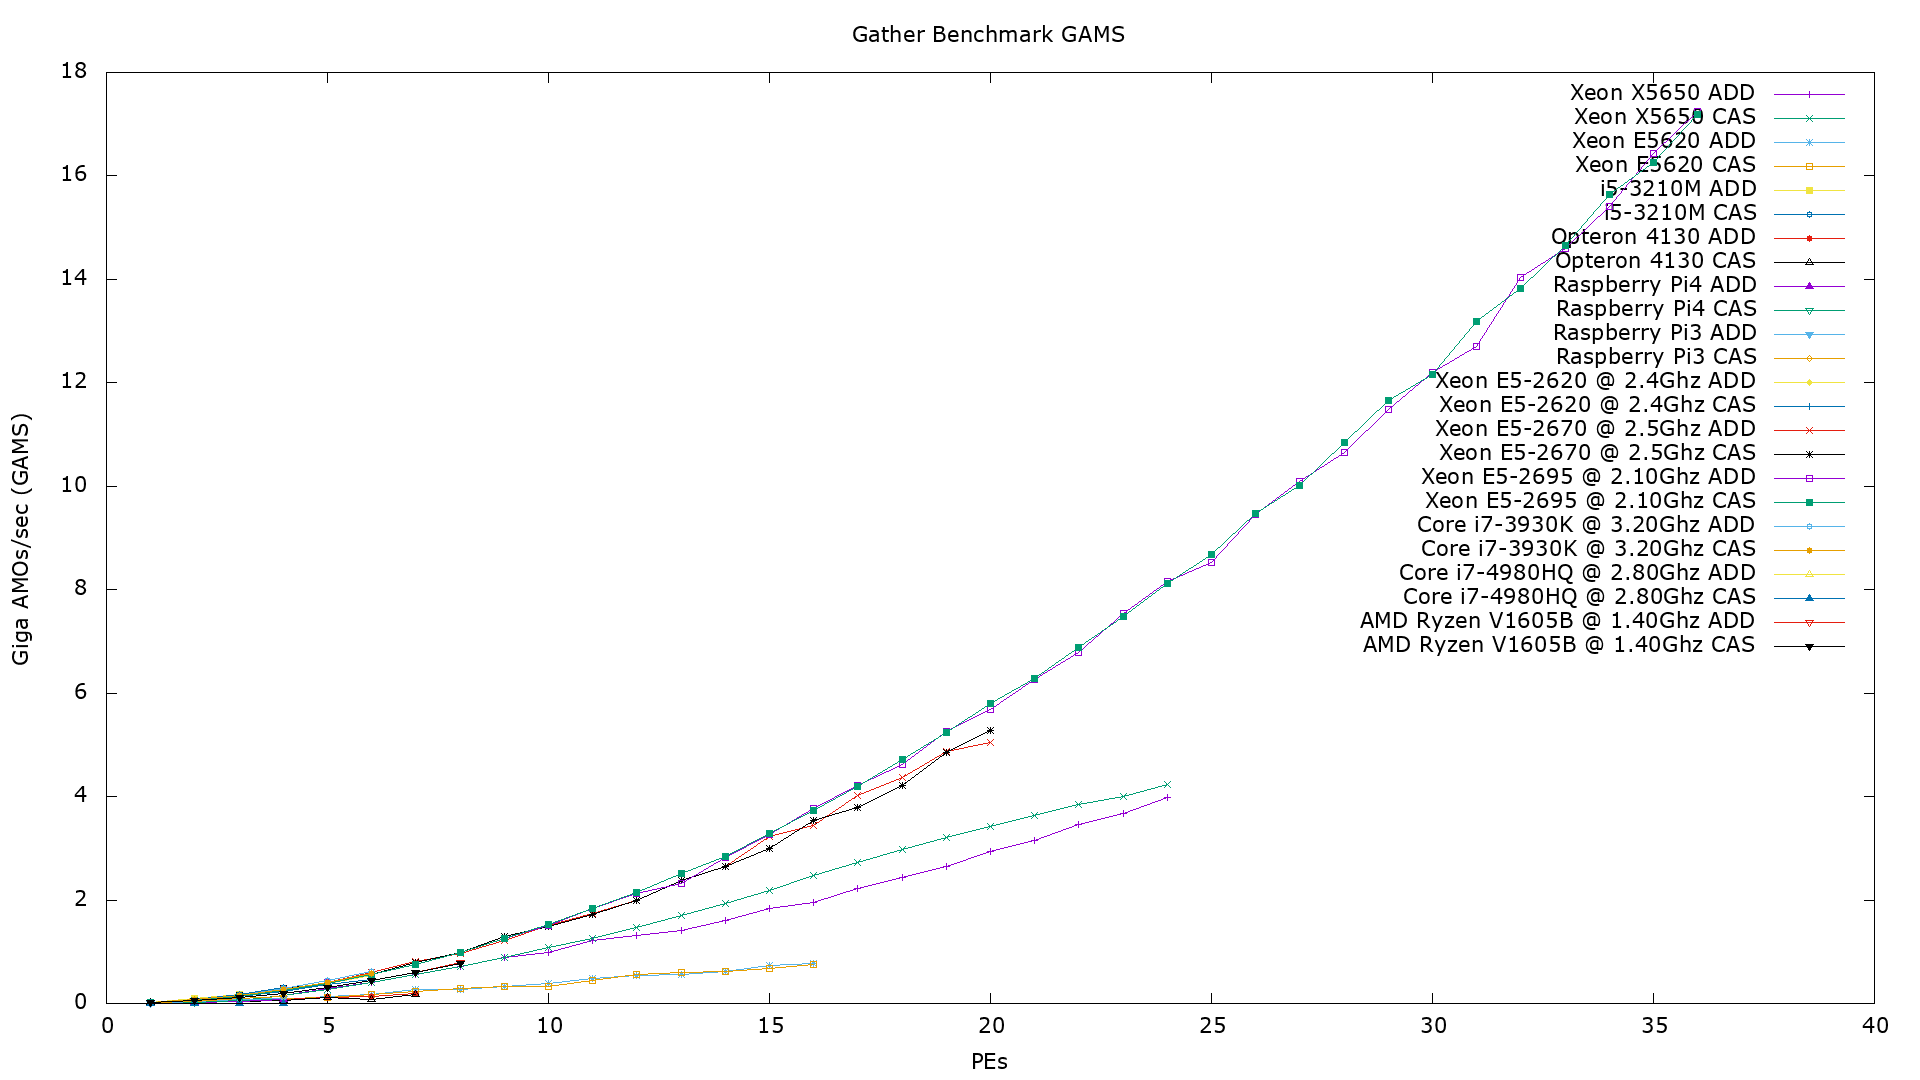
\includegraphics[width=3.5in]{figures/GATHER_GAMS.png}
\caption{Gather Benchmark GAMS}
\label{fig:gather_gams}
\end{figure}

\begin{figure}[!t]
\centering
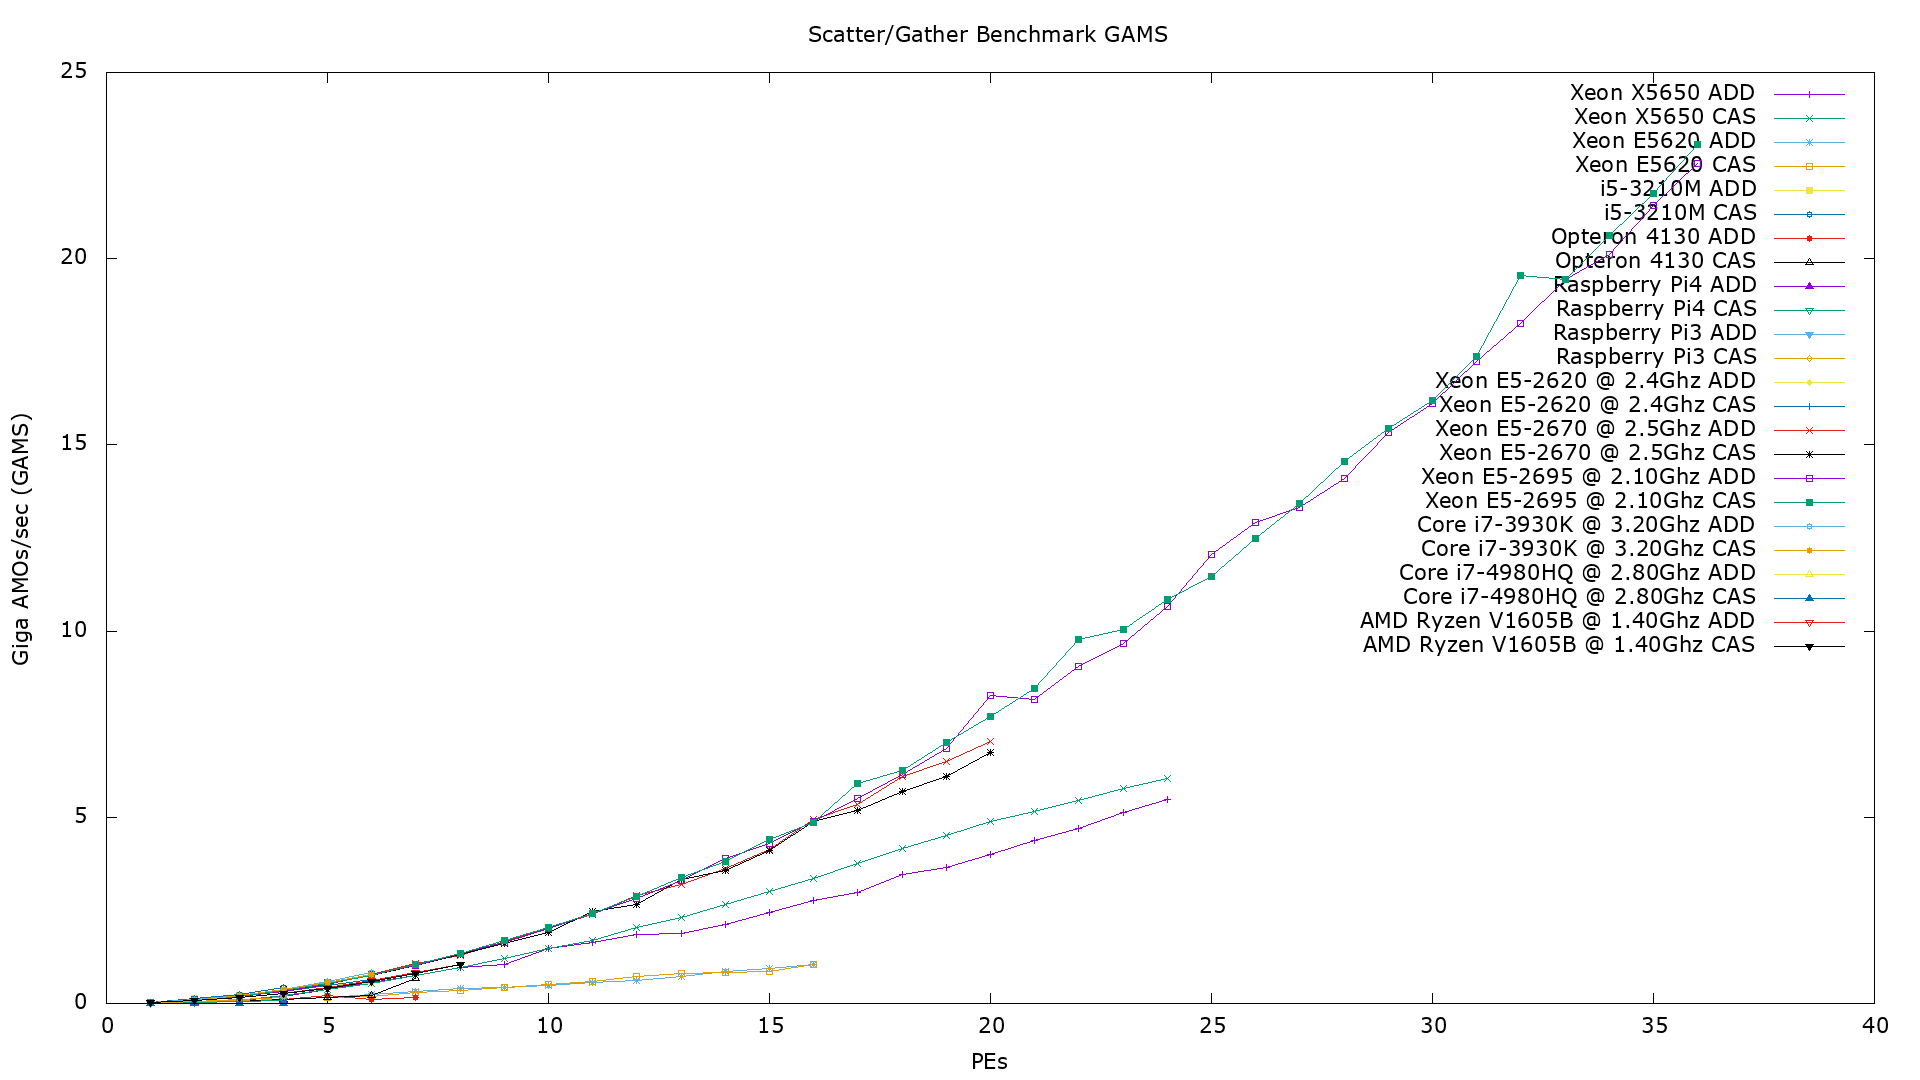
\includegraphics[width=3.5in]{figures/SG_GAMS.png}
\caption{Scatter/Gather Benchmark GAMS}
\label{fig:sg_gams}
\end{figure}

\begin{figure}[!t]
\centering
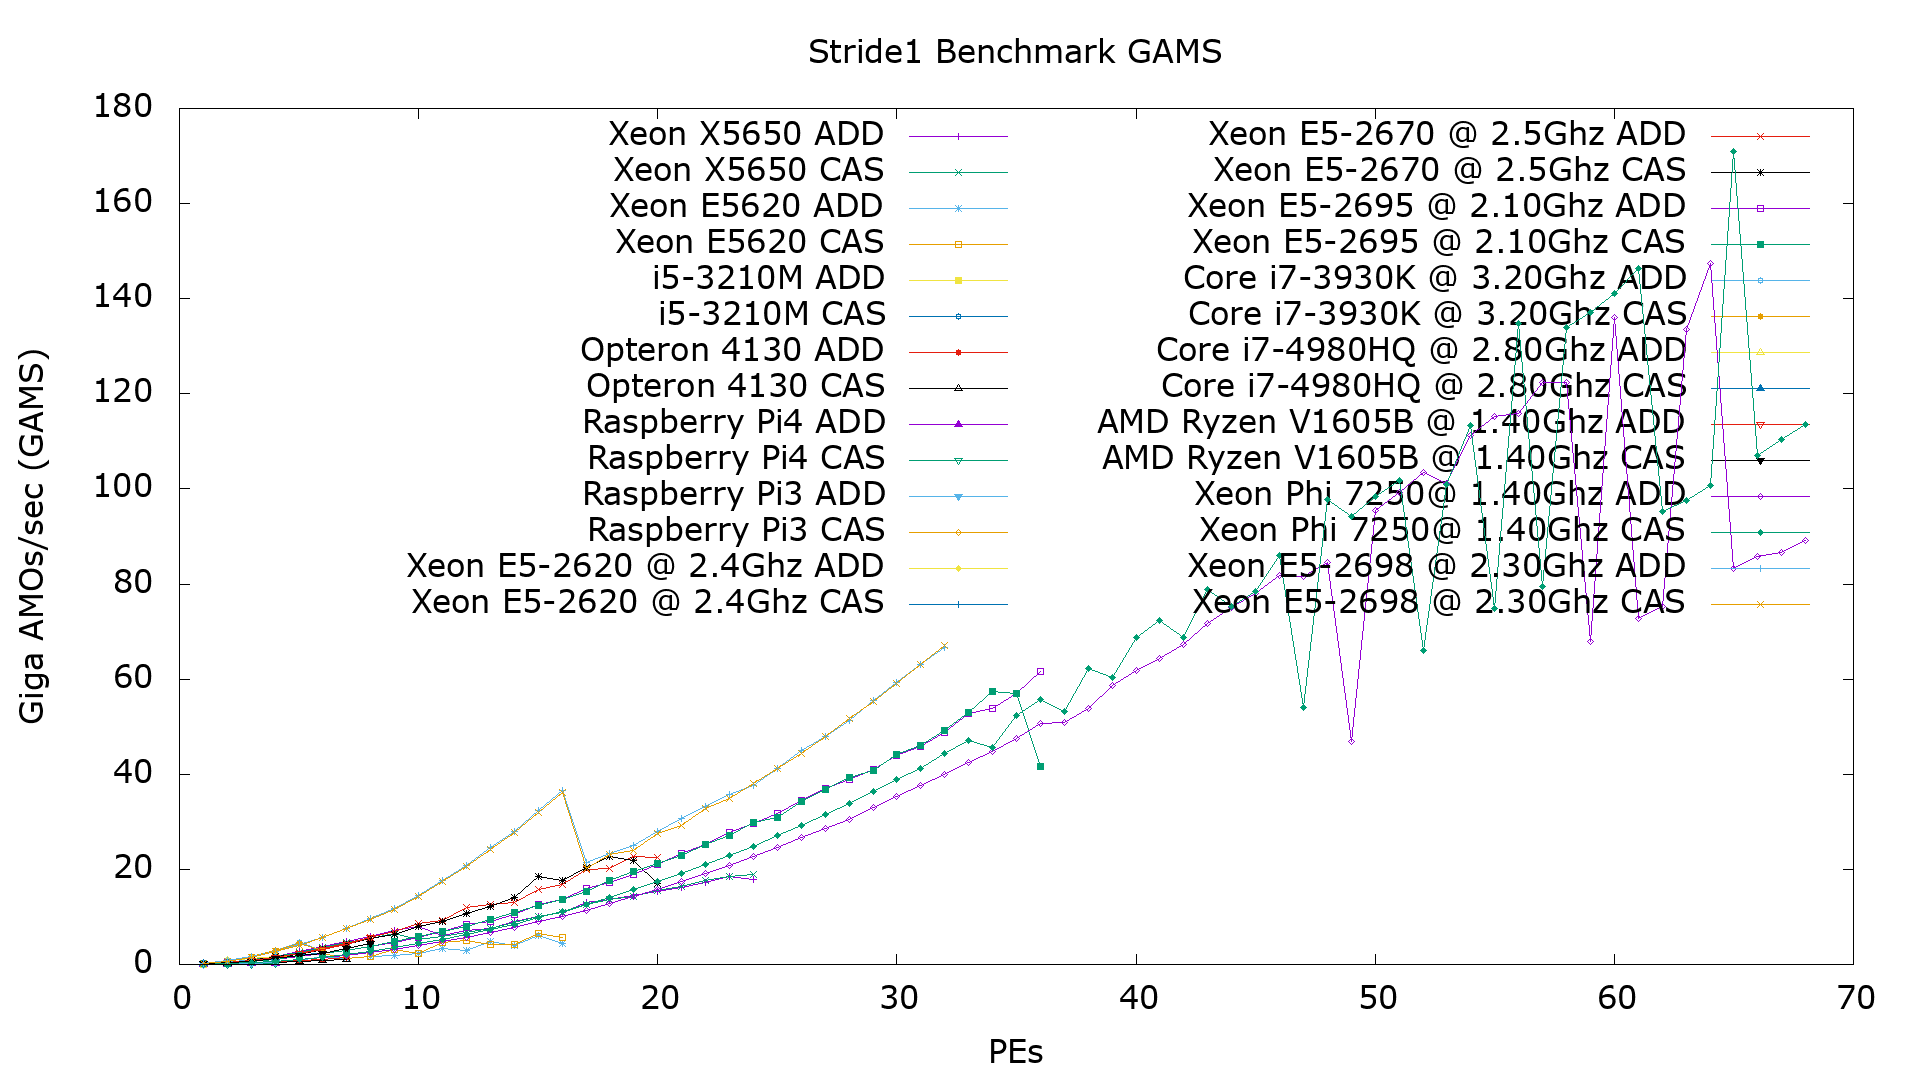
\includegraphics[width=3.5in]{figures/STRIDE1_GAMS.png}
\caption{Stride-1 Benchmark GAMS}
\label{fig:s1_gams}
\end{figure}

\begin{figure}[!t]
\centering
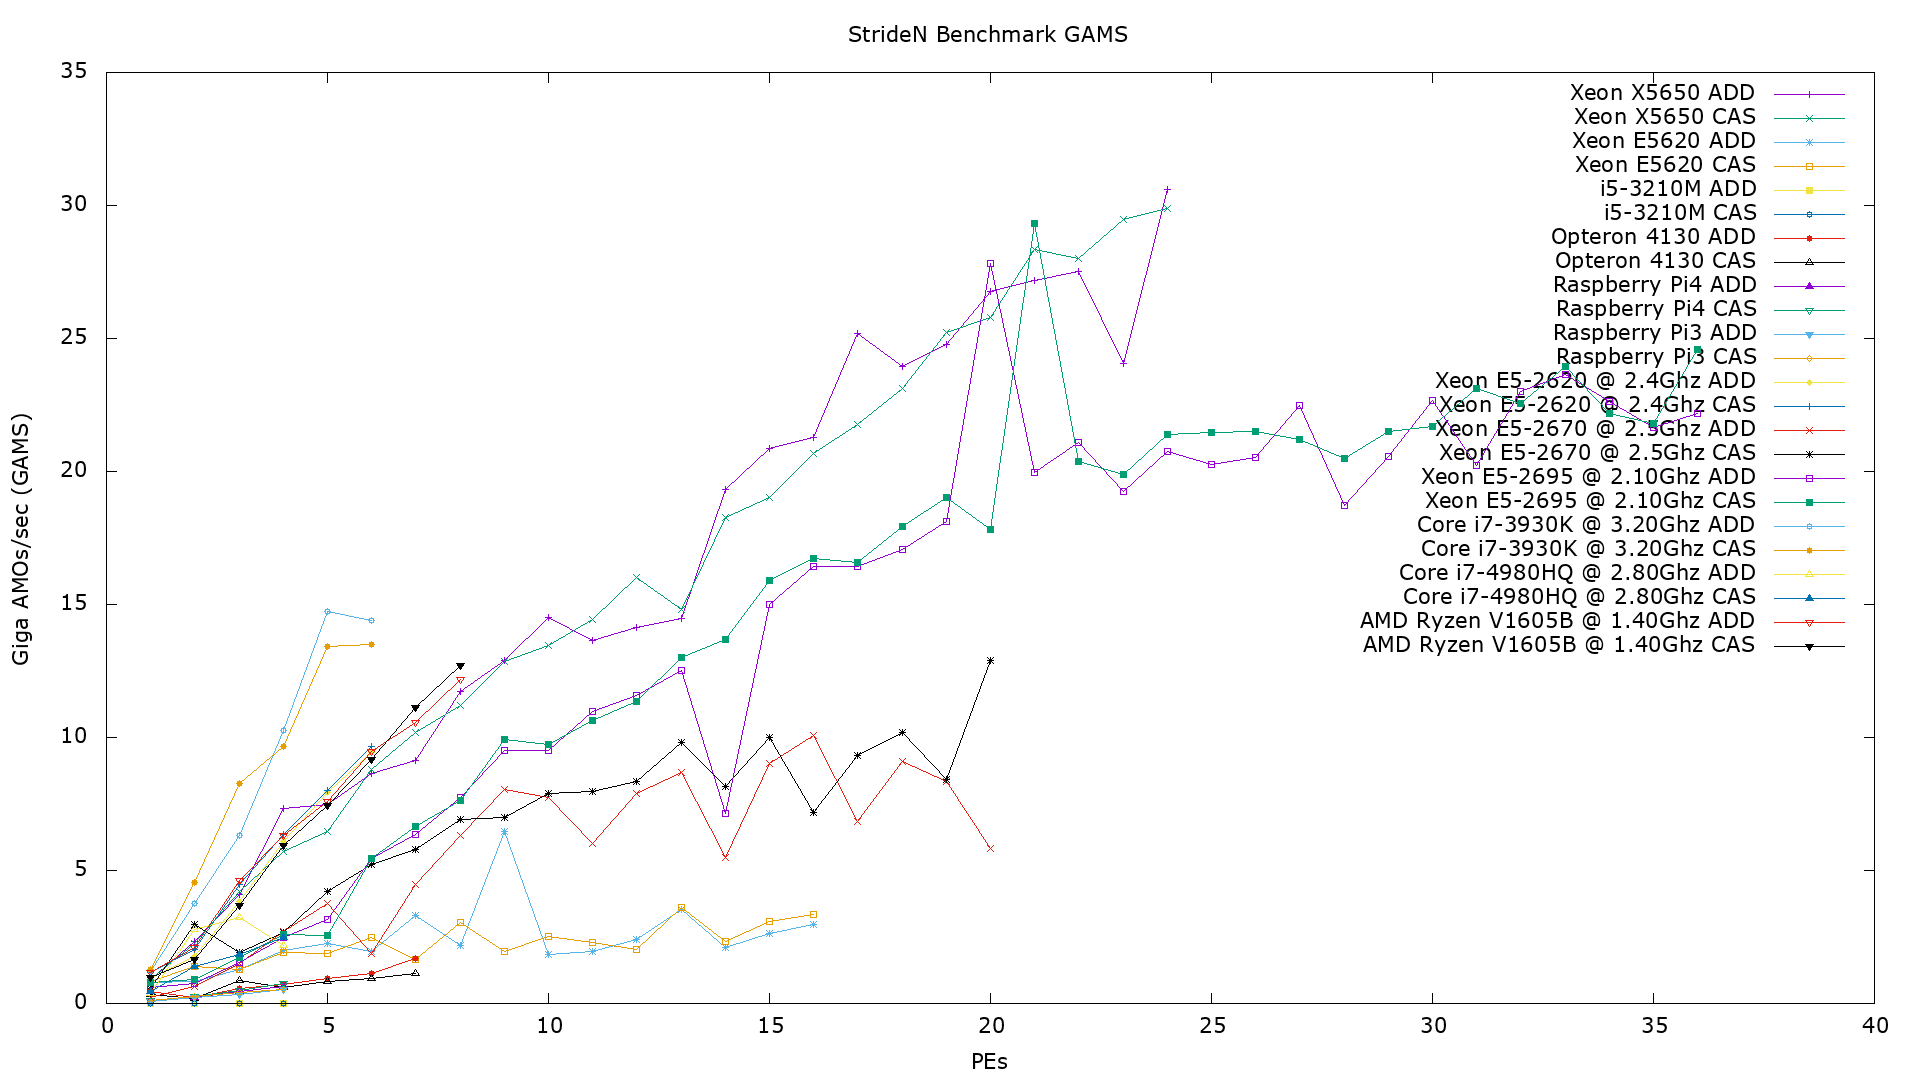
\includegraphics[width=3.5in]{figures/STRIDEN_GAMS.png}
\caption{Stride-N Benchmark GAMS}
\label{fig:sn_gams}
\end{figure}
